\section{Poincar\'e Maps}
Since plots of invariant manifolds in configuration space can be complex and do not display any
velocity information about the trajectories, a different visualization technique is advantageous.
Poincar\'e mapping is an approach that concisely visualizes trajectories by reducing the dimension
of the problem through an intersection surface. These surfaces can be physical, like a plane or
sphere in configuration space, or more abstract, like an apse or velocity map. As initial
conditions are propagated, whenever a trajectory passes through the surface, its crossing is
marked on the Poincare\'e map. A simple example appears in \cref{fig:map}. The mapping technique
provides an intuitive representation of complex trajectory behaviors, aiding in the analysis and
interpretation of manifold dynamics.

\begin{figure}[H]
    \centering
    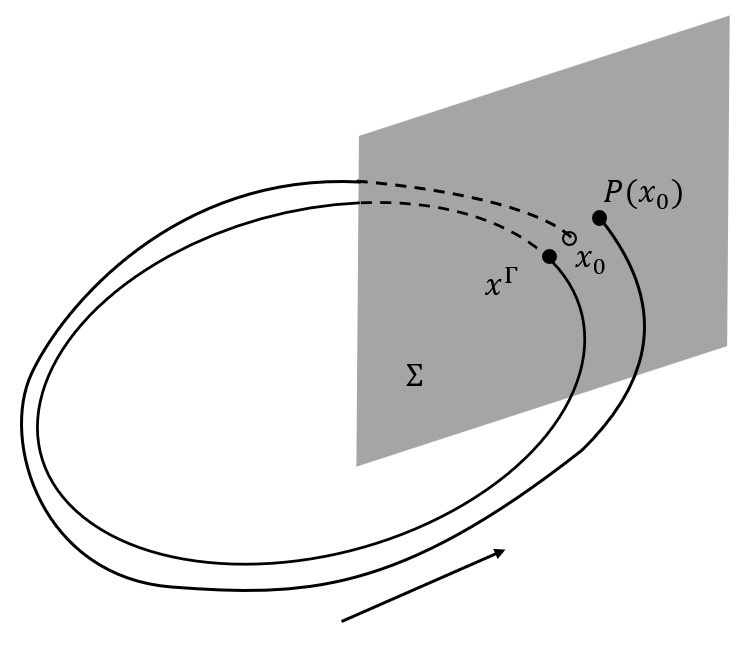
\includegraphics[width=0.5\textwidth]{figures/Map.jpg}
    \caption{Poincar\'e map.}
    \label{fig:map}
\end{figure}

Poincaré mapping provides a powerful method for visualizing and analyzing trajectory behavior by
reducing the dimensionality of the problem through surface intersections. Starting from an initial
condition $x_{0}$ on the intersection surface $\Sigma$, after propagation, the trajectory returns
to the surface at $P(x_{0})$. If the trajectory is precisely periodic, the trajectory returns to
the same point, $x^{\Gamma}$. The Poincar\'e map then is the 2-dimensional representation of the
surface, displaying only the trajectory crossings. Note that the axes of the map need not be
position components but could also be velocity, energy, etc. Similar mappings are employed in this
investigation to more efficiently analyze and compare different trajectories.
